\documentclass{standalone}
\usepackage{tikz}
\usetikzlibrary{arrows.meta}
\begin{document}
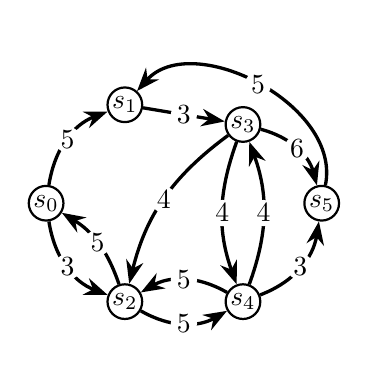
\begin{tikzpicture}
    \begin{scope}[every node/.style={circle,thick,draw, inner sep=0.6pt}]
        \node (s0) at (0,0) {$s_0$};
        \node (s1) at (1,1.25) {$s_1$};
        \node (s2) at (1,-1.25) {$s_2$};
        \node (s3) at (2.5,1) {$s_3$};
        \node (s4) at (2.5,-1.25) {$s_4$};
        \node (s5) at (3.5,0) {$s_5$};
    \end{scope}
    \begin{scope}[
        every node/.style={fill=white,circle, inner sep=0.5pt},
        every edge/.style={-{Stealth[]},draw=black,very thick}]
        \path[->] (s0) edge[bend right=30] node {$3$} (s2);
        \path[->] (s1) edge node {$3$} (s3);
        \path[->] (s4) edge[bend right=30] node {$3$} (s5);
        \path[->] (s3) edge[bend right=20] node {$4$} (s2);
        \path[->] (s3) edge[bend right=20] node {$4$} (s4);
        \path[->] (s4) edge[bend right=20] node {$4$} (s3);
        \path[->] (s0) edge[bend right=-30] node {$5$} (s1);
        \path[->] (s2) edge[bend right=20] node {$5$} (s0);
        \path[->] (s2) edge[bend right=30] node {$5$} (s4);
        \path[->] (s4) edge[bend right=30] node {$5$} (s2);
        \path[->] (s5) edge[bend right=75] node {$5$} (s1);
        \path[->] (s3) edge[bend right=-30] node {$6$} (s5);
    \end{scope}
\end{tikzpicture}
\end{document}